\section{Estado del arte}
\label{sec:StateOfTheArt}


\subsection{Eventos}
Un evento es una notificacion de que algo ha ocurrido. Es mayormente utilizado
para mantener comunicaciones 1 a n, sin tener acoplamiento.

En la contruccion de interfaces de usuario, se utilizan los eventos para 
manejar la comunicación del dominio con la interfaz.

\bigskip

Existen varias formas de manejar la comunicación entre el dominio y la vista. 
A continuación detallaremos las formas más comunes de realizar la comunicacion:

\begin {enumerate}

	\item {\bf Implicita} Donde los objetos de dominio tienen que
	 lanzar explicitamente un evento cada vez que el valor de una propiedad cambia,
	 como lo hace JFace-DataBinding y el Arena actual.
	\cite{sousa00formal}
	La forma que tienen para dar el sopote de eventos es utilizando un
	\emph{PropertyChangeSupport}, que registra a los listener y les notifica el que
	el objeto de domino cambio el valor de alguna propiedad.
	
	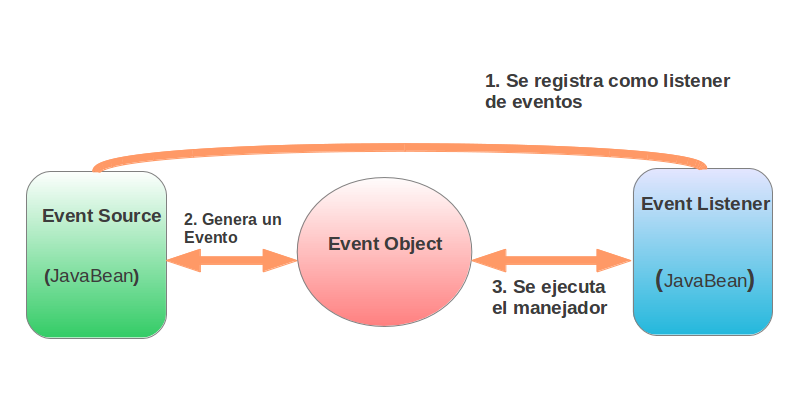
\includegraphics[width=350px, height=200px]{img/javabeans}
	
	\bigskip
	
	\item {\bf Web Form} A través del submmit de un formulario. Wicket es
	un Framework web MVC para Java. Su sistema de binding  es a través de submit de un
	formulario, eso trae dos implicaciones:
	 
		\begin {enumerate}
		
			\item{\bf Submit con Refresh}  EL dominio no tira eventos, en el momento de
			renderizar la página se leen nuevamente todas las propiedades del dominio.
			Como wicket corre sobre una plataforma web, en el form vuelve a enviar toda
			la pagina, y al volver, la renderiza nuevamente.
			
			Por otro lado, tampoco es necesario tener eventos desde la vista hacia el
			modelo. El concepto de Form decide qué datos son los que hay que volcar de un
			lado a otro.

			\item {\bf Submit con Ajax} 
			Es una derivación del alterior, a diferencia de que solo se envía
			una porcion de la página, entonces hay que decirle explicitamente que parte
			de la pagina queremos refrescar, para que solo renderice esa parte.
		
		\end {enumerate}
		
		
	\item investigar que hace morphic, preguntar a Guille.
	Y tal vez otros frameworks\ldots acá preguntémosle a Javi otros modelos de
	binding.
\end{enumerate}	


\subsection{Transacciones}

En esta seccion analizaremos las propiedades ACID en las interfaces de usuario.


{\bf Soluciones comunes:}

\begin {itemize}

\item Patrón: Objetos de transacción
\item Unidad de trabajo
\item Clonar al editar
\item Transacciones de Base de datos 
\end {itemize}

\begin {itemize}

\item {\bf Objetos de transacción}
Provee una interfaz separada para las transacciones en el contexto de capas de
acceso a bases de datos.\\
{\bf Solución} Utilizar un objeto de transacción. Hay que hacer rollback en el
destructor, para que las transacciones abiertas sean abortadas.

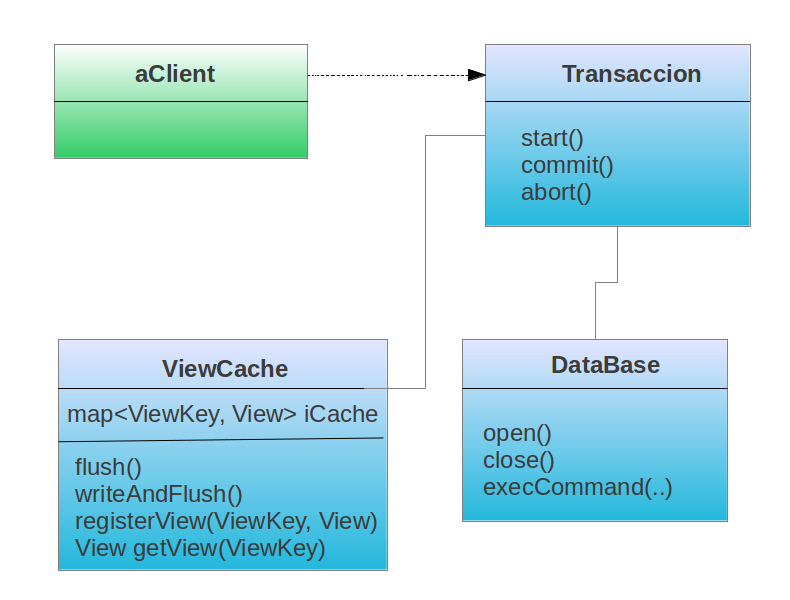
\includegraphics[width=300px, height=200px]{img/objectTransaction}

\item {\bf Unidad de trabajo }
Mantiene una lista de objetos afectados por una transacción de negocio y
coordina los cambios de escritura y la resolución de problemas de concurrencia.
Una unidad de trabajo realiza un seguimiento de todo lo que haces durante una
transacción que puede afectar a la base de datos. 
Cuando haya terminado,impacta todos los cambios en la base de datos.

\item {\bf Clonar al editar}
Esta solución es bastante común. En el momento que se quiere editar un objeto,
se lo clona, y se modifica el objeto clonado. Cuando se confirma la edición, se
impacta los cambios del clon en el objeto original.

\item {\bf Transacciones de base de datos}
Con este sistema, al momento de edición del objeto, se crea una transacción en
la base de datos, y en la confirmación de la edición, se comitea la transacción.
Y si se quiere cancelar, se hace un rollback en la transacción y los cambios se
revierten.

\end {itemize}

